\section{Thesis Outline}\label{sec:intro_thesis_outline}

In this section, the observed challenges from the state of the art in the area are defined and which are possible proposals to solve them. Based on this, the thesis objectives to go beyond the state of the art are defined. At the end, the research lines to attains these goals are described. The particular contribution of each paper of the thesis and its related publications are detailed in Section~\ref{sec:contributions}.

\subsection{Challenges in the State of the Art}
Currently from the state of the art, different problems were identified from both prior work and observations during the thesis. Therefore, we describe the major challenges that were reviewed and addressed during this research. 

\subsubsection{1. Cloud Sizes: From Unicast D2D Pairs to Multicast D2D Clouds}
\label{sec:cloud_sizes}

From the state of the start, prior works have considered that the short-range communications utilizes unicast pair of devices to offload the mobile network. To observe potential benefits in these scenarios, it was investigated the possibility of multicasting with more devices inside the mobile cloud to cooperate. In Fig.~\ref{fig:cloud_sizes}, it is presented the benefits of increasing the amount of devices that cooperate to share the content.

\begin{figure}[h]
  \centering
  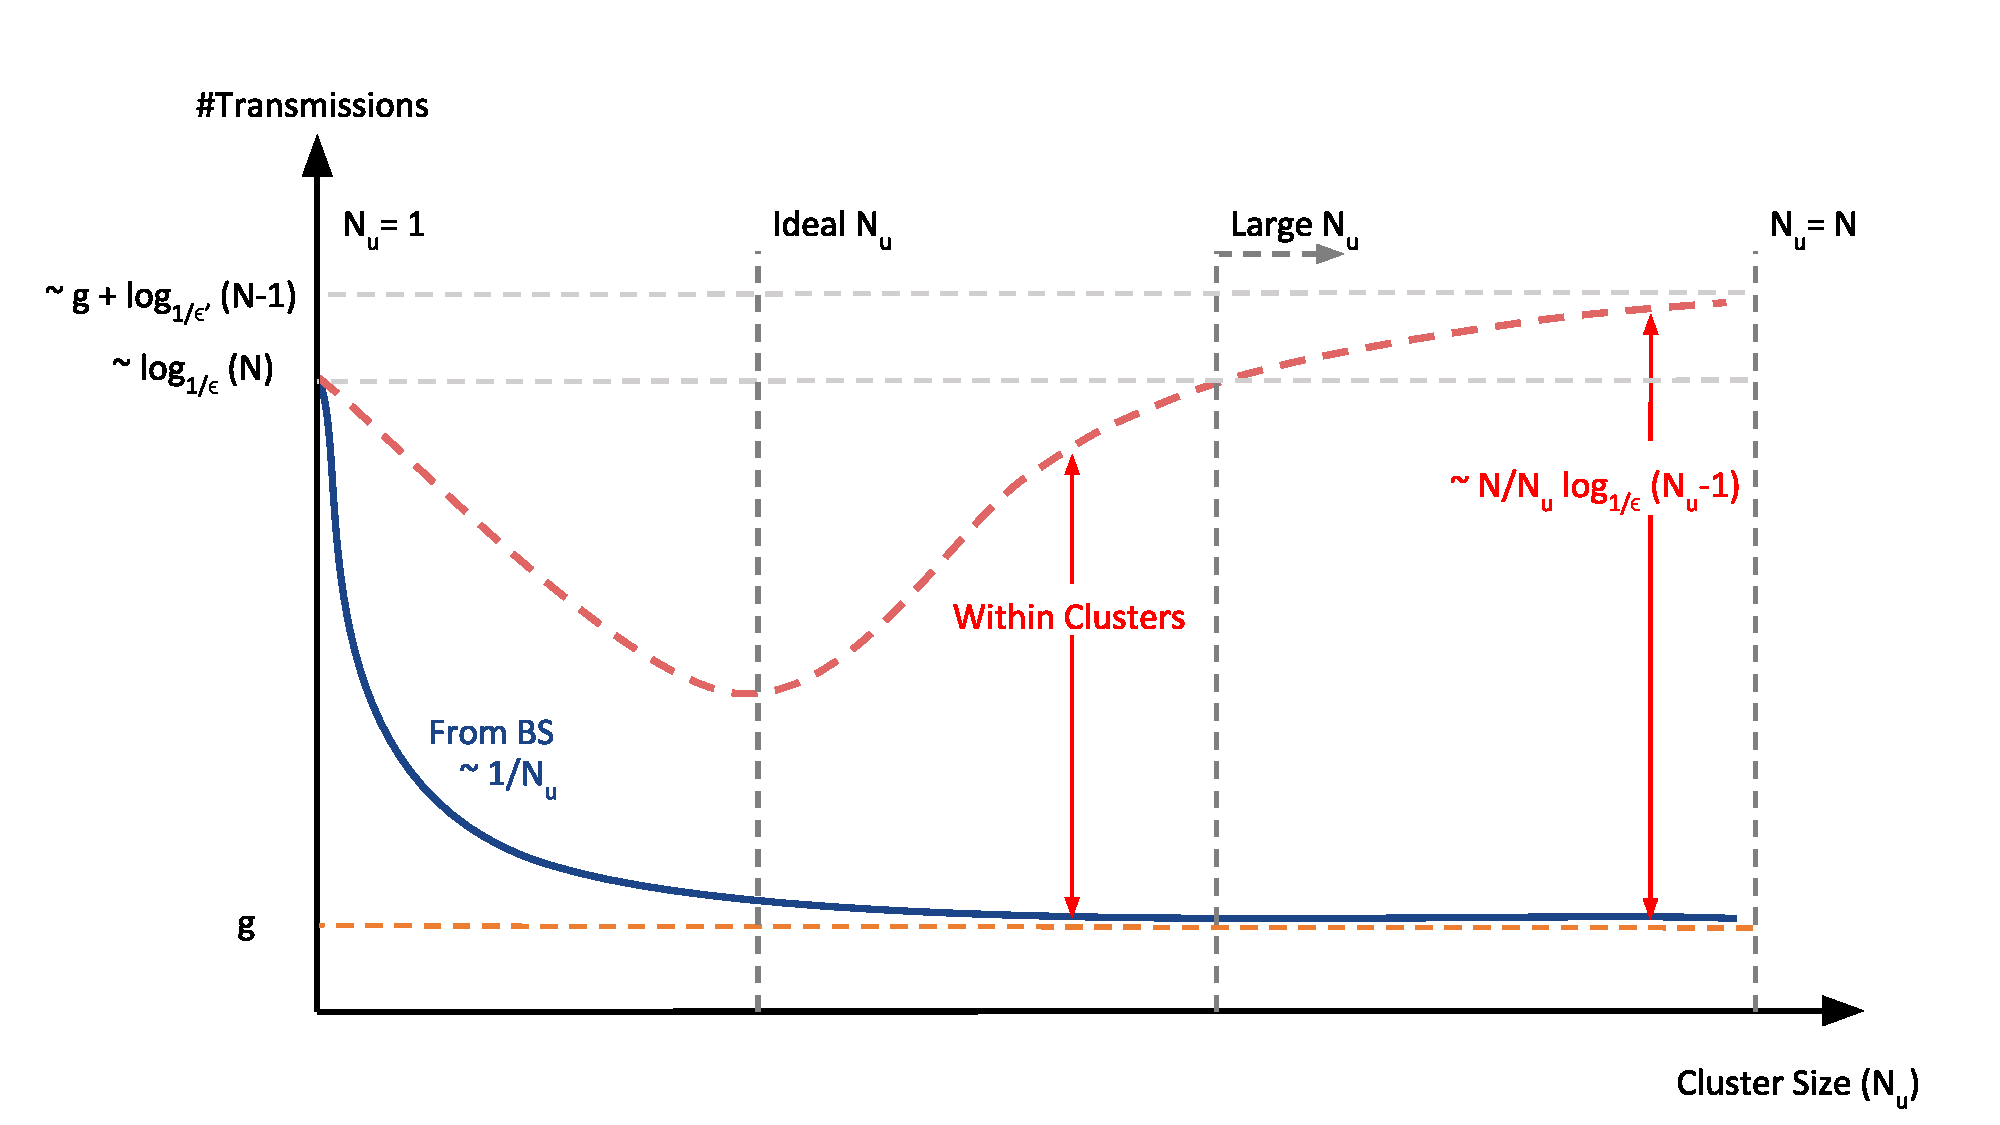
\includegraphics[width=\textwidth]{introduction/figures/cloud_sizes.pdf}
  \caption{Total number of transmissions trends vs. Cluster size.}
\label{fig:cloud_sizes}
\end{figure}

The figure considers a scenario similar to the presented in Fig.~\ref{fig:cooperation}. It indicates the mean total number of transmissions required to decode a batch of $g$ packets coded with \ac{RLNC} in a multicast network of a \ac{BS} and $N$ devices vs. the number of devices cooperating inside each cluster (cloud size) $N_u$. Thus, there are $\lceil \frac{N}{N_u} \rceil$ clusters and $1 \leq N_u \leq N$. This figure presents the spectrum of cooperation since $N_u = 1$ represents broadcast or no cooperation, $N_u = N$ represents full cooperation of one cloud with all the devices and all other cases represents variable degrees of cooperation of various clouds with some devices.

For this reference scenario, it is assumed that all the packet erasures are independent and identically distributed. Also, all the devices present the same packet erasure probability $\epsilon$ for simplicity. It is also assumed that all devices have connectivity with the \ac{BS} and are fully connected through an short-range orthogonal communications channel, e.g. \ac{D2D}, \ac{WiFi} network, etc. The packet erasures of the links inside the cloud are also independent and identically distributed with probability $\epsilon'$. Also, we consider the case where $N \gg g$.

After some transmissions have been made from the base station, the devices share locally coded (or recoded) packets in rounds with broadcast with \ac{RLNC} in a coordinated fashion. The orthogonal channel is used to recover from the packet erasures when the \ac{BS} transmitted. By reviewing the scaling laws of this metric in \cite{eryilmaz2008delay} and analyzing this scenario, some trends can be obtained.

First, the mean total number of transmissions of broadcast with \ac{RLNC} of $N$ devices, homogeneous packet erasure probability $\epsilon$ and $N \gg g$ scales as $\log_{\frac{1}{\epsilon}}(N)$ \cite{eryilmaz2008delay}. This is the value at $N_u = 1$. Second, The blue curve models the mean number of transmissions that the \ac{BS} makes. As $N_u \rightarrow N$, the number of transmission from the \ac{BS} approaches to the bare minimum $g$. This occurs because the probability of not receiving a packet in a cloud is ${\epsilon}^{N_u}$, which vanishes rapidly for increasing $N_u$. Third, The red dashed curve stands for the total number of transmissions of the devices. This curve accounts for both the transmissions from the \ac{BS} and inside each cloud. When the clouds are small, the amount of transmissions from the \ac{BS} diminish more rapidly than the amount of transmissions inside each cloud. However, after some amount of devices per cloud, adding more devices does not reduce the amount of transmissions from the \ac{BS} significantly. Instead, this only increases the amount of transmissions within the clouds. As $N_u \rightarrow N$, the total number of transmissions of the devices approaches to the maximum possible, $ g + \log_{\frac{1}{\epsilon'}}(N - 1)$ since at least one device is transmitting at every round.

Currently, the state of the art considers using either $N_u = 1$ or $N_u = 2$ since it is not considered to multicast from the devices. More important, from Fig.~\ref{fig:cloud_sizes} it can be observed that an optimal cloud size exists to reduce the number of transmissions. This value also represents the operational point of highest throughput and lowest energy consumption vs. other designs with different cloud size. Therefore, the regimes and conditions to achieve these values were be investigated.

\subsubsection{2. RLNC Performance Parameters: Design Trade-Off}
\label{sec:rlnc_trade_off}
There has been different studies that addressed the impact of \ac{RLNC} parameters in its performance, i.e. the generation size $g$ and the field size $q$, in both theoretical and practical applications with mobile devices\cite{heide2009network,lucani2009random,heide2011code,trullols2011exact,zhao2012notes,paramanathan2013lean}. The generation size affects the algorithmic complexity of both encoding and decoding. The computational complexity of \ac{RLNC} scales as $\mathcal{O}(g)$, i.e. linear. For the decoding, Gaussian elimination is of cubic complexity $\mathcal{O}(g^3)$ in principle, given the inversion of a square matrix of size $g$. However, a structured Gaussian elimination implementation can achieve $\mathcal{O}(g^2)$ for $g < 512$ as reported in \cite{paramanathan2013lean}. Given that the field size effects are diverse, these are resumed in Table~\ref{tab:rlnc_parameters}.

\begin{table}[h]
  \centering
  \caption{Field size effects in the code performance.}
  \begin{tabular}{|M{0.75cm}|M{2cm}|M{1.5cm}|M{2.65cm}|M{2cm}|}

    \hline
    $q$         & Linear Dependency & Signalling & Overhead Major Contributor & Field Complexity  \\
    \hline
    \hline
    $< 2^8$     & High       & Low        & Linear Dependency & Low \\
    \hline
    $\geq 2^8$  & Low        & High       & Signalling & High \\
    \hline

  \end{tabular}

\vspace{0.2cm}
\label{tab:rlnc_parameters}
\end{table}

Table~\ref{tab:rlnc_parameters} shows the effects of the field size for two principal regions: low and high field sizes. The criteria to separate them has been to consider a field size as high for values higher than $2^8$ for reasons that will be explained below. The table also displays various metrics to evaluate the performance of the code.

Linear dependency refers to the amount of linearly dependent coded packets that are generated during the transmission process. As more linearly independent coded packets are received during the transmission process, linearly dependent coded packets are generated more frequently towards the end of the transmission. Dependent packets are useless since they provide no new information to the decoder and are discarded. Once $g - 1$ independent coded packets have been received, the probability of generating a dependent coded packet is $\frac{1}{q}$ \cite{lucani2009random,trullols2011exact,zhao2012notes}. For the binary field, i.e. $GF(2)$, there is a 50\% probability of generating useless packets. In the case of $GF(2^8)$, this probability reduces to less than 0.5\% making it depreciable in practice. In terms of the generation size, the linear dependency effect can be observed on the average amount of transmissions for decoding. For $GF(2)$, $g + 1.667$ transmissions on average are required to decode the original set, whereas for $GF(2^8)$ this value can be approximated to $g$ for practical purposes. 

Signalling is interpreted as the amount of bits required to represent the coding coefficients. These bits are attached to each coded packet and for each original packet \cite{heide2011code}. We referred to this value previously as $|v_{i}| = g \times \log_{2}(q)$ which grows linearly with $g$ and logarithmically with $q$. For $GF(2)$, only 1 bit per packet is required to be included in each coded packet to signal the coding coefficients. However, for fields such as $GF(2^8)$ or higher, more than one byte is necessary for each original packet to signal its coding coefficients. Therefore for high generation sizes, high fields could potentially make the amount of signalling even higher than the original packet size.

Thus, overhead accounts for both effects of the linear dependency and coding coefficients signalling respect to useful data. In Table~\ref{tab:rlnc_parameters}, it has been specified which is the effect that accounts for most of the total overhead in the specified region. For low fields, most of the overhead comes from linear dependency effect , but for higher field sizes the signalling from the coding coefficients becomes critical. 

Finally, field complexity accounts for the computational cost and time required for the operations in \ac{GF} arithmetics required to process the data. Besides algorithmic complexities, the field utilized to operate on the data affects the code performance in terms of time and energy spent on processing. The binary field poses a low computational burden on the device carrying the operations since modulo-2 operations are XOR/AND operations. However, increasing the field size requires to define and operate with new arithmetics which incur in higher processing times. Thus, a proper field size for mobile devices is important to ensure a satisfactoring code processing speeds \cite{heide2009network,paramanathan2013lean}.

In terms of mobile applications, all of these aspects relate to the application throughput and energy consumption. Ideally, parameter configurations that achieve: (i) low number of transmissions required to decode, (ii) low total overhead and (iii) low field complexity are desirable. Such code performance metrics would lead to the goal of high throughput and low energy consumption at the mobile devices and the \ac{BS}. However, as seen from the previous description, these objectives are conflictive posing a \textit{trade-off} for using only \ac{RLNC} in our scenario. Since most of the state of the art in the area considers \ac{RLNC} as its erasure correcting code, other code constructions that avoid the presented trade-off should be considered in order to achieve the previous goals.

\subsubsection{3. Evaluation of Transmission Policies in Wireless Local Area Networks}
In order to obtain ideal rules to choose ideal transmitters in multicast with \ac{RLNC}, the works in \cite{khamfroush2013minimizing,khamfroush2015optimal,khamfroush2014coded} have evaluated the cases of: (i) multicasting to \ac{D2D} cooperative pairs and (ii) multicasting to a pair of nodes sharing a unidirectional unicast link in the presence of interferers. In both works, the theoretical problem of finding the ideal policy reduces to solving a \ac{MDP}. However, this type of problems pose a computational burden that is unfeasible in real networks, thus requiring the application of heuristics that are evaluated self-defined numerical simulators or even implementations. Using these kind of tools could potentially not be maintenable or reusable slowing the design process of the protocol developers. Moreover, these protocols assume that the devices have been assigned orthogonal communication resources. Nevertheless, in scenarios of this type, devices may access the medium in an uncontrolled manner thus requiring the evaluation of a decentralized access method.  

\subsection{Objectives}
Based in the previous challenges, this thesis pushes the state of the art by using multicast \ac{D2D} mobile clouds in cooperative wireless networks with \ac{RLNC} since current techniques focuses mostly in \ac{D2D} communications based in unicast pairs with either \ac{RLNC} or non-composable rateless codes. Therefore, the objectives of this thesis are to:

\begin{enumerate}

\item Define the regions and conditions in terms of the code parameters; and energy, data rate costs where cooperation with \ac{RLNC} provides a better performance than broadcast with \ac{RLNC} in terms of data throughput and energy consumption at the \ac{BS} and mobile devices.

\item Study the dominating regimes and ideal cloud sizes to observe if there exists ideal values for high system throughput and low energy consumption as described in Section~\ref{sec:cloud_sizes}.

\item Propose and study code constructions that overcome the \ac{RLNC} trade-off and achieve the goals described from Section~\ref{sec:rlnc_trade_off}. In this sense, the objective is to find codes that permit to retain the low coding coefficients overhead from a low field size, but also the low number of transmissions overhead from high fields.

\item Study the effect of transmission policies under a \ac{WLAN} scenario in an easy-to-deploy manner. In this case, medium access mechanisms to avoid interference should be considered. Also, the use of standard simulation tools that are reusable for the research community and well maintenated is desired.

\end{enumerate}

\begin{figure}[h]
  \centering
  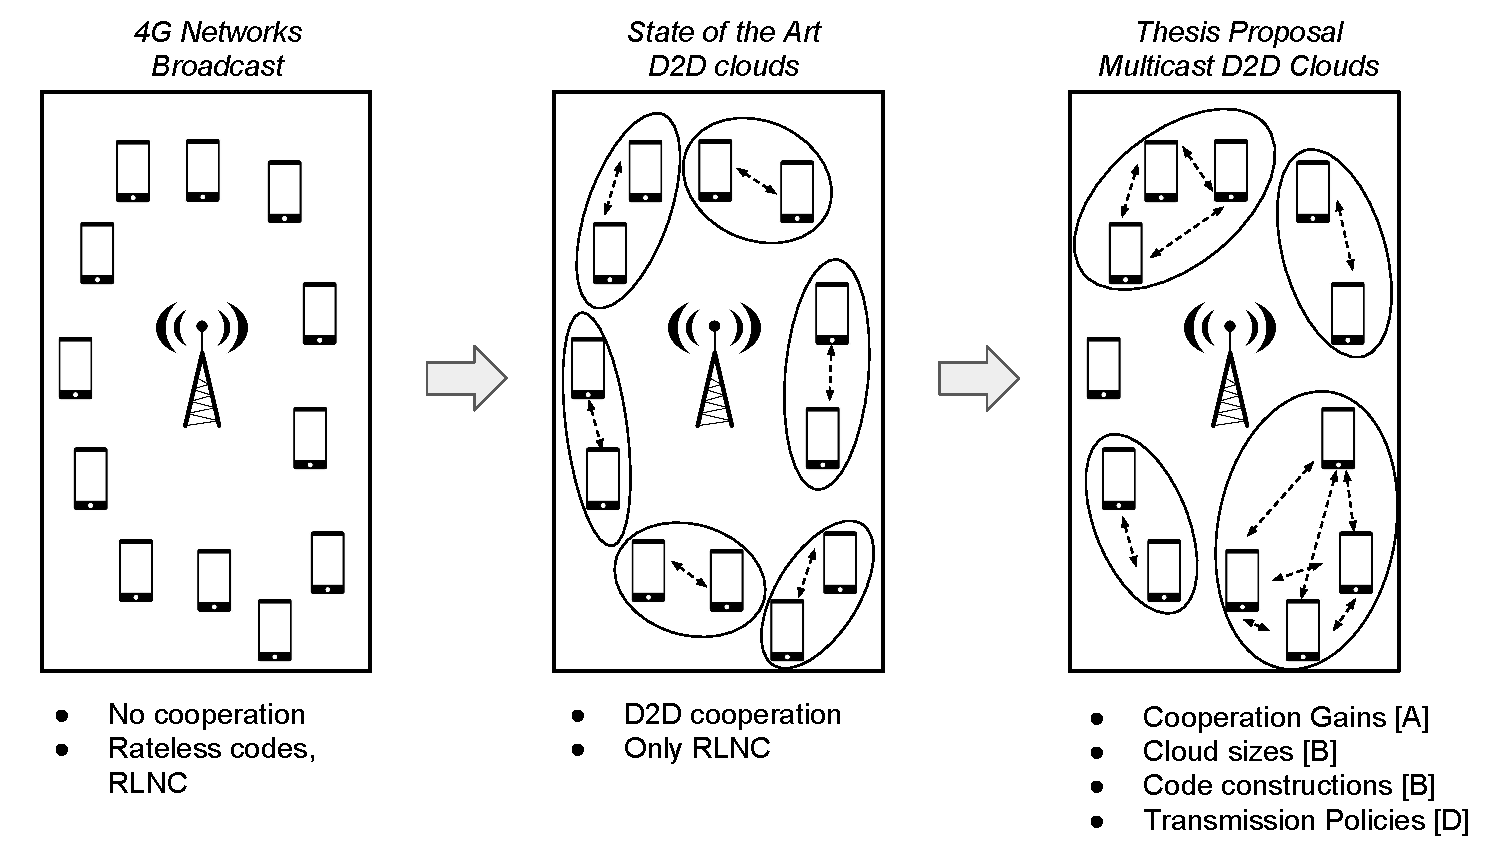
\includegraphics[width=\textwidth]{introduction/figures/thesis-diagrams.pdf}
  \caption{State of the Art and Thesis Proposal.}
\label{fig:proposal}
\end{figure}

From Fig.~\ref{fig:proposal}, the study for objective 1 was addressed in paper {[\ref{paper:paperA}]}. Objectives 2 and 3 were reviewed in paper {[\ref{paper:paperB}]}. Finally, objective 4 was addressed in paper {[\ref{paper:paperD}]} with a software tool implemented in paper {[\ref{paper:paperC}]} that uses Kodo and the open-source ns-3 simulator \cite{ns3link}.

\subsection{Research Lines}

Based on the concepts of multicast \ac{D2D} communications with \ac{RLNC} in cooperative wireless networks, this thesis covers two outlines. First, it was considered a research line which its main goal was to obtain network codes for cooperation in underlay \ac{D2D} cellular networks to enhance the throughput and reduce the energy consumption but also minimize the total overhead from the \ac{BS} and the mobile devices. Here, \ac{D2D} communications take place within the cellular spectrum between mobile devices in the same cell and the interference is prevented under pre-defined network planning. Second, a research line to investigate the transmission policies for mobile devices in a decentralized multihop \ac{WLAN} was considered to enhance the previously mentioned metrics by reducing the required number of transmissions to decode a batch of packets. At the end, network coded cooperation in multihop networks and \ac{D2D} communications are combined to give data services to the end-user.

\subsubsection{1. Network Code Constructions and Regimes in Multicast Cooperative D2D Cellular Networks}

Given the increase of data rates in cellular networks such as \ac{LTE-A}, we first addressed the question of when is it reasonable for a set of devices to cooperate when downloading a multicast content. The underlying reason is that there has been improvements on the cellular data rates that had approached them to the order of \ac{WLAN} data rates. Thus, in paper {[\ref{paper:paperA}]}, we investigated which are the regions where cooperation with \ac{RLNC} achieves a better perfomance than broadcast with \ac{RLNC} in terms of the throughput and energy costs. From this work, we observed that codes with high field size provided a reduced amount of transmissions translating into a high throughput but at the expense of including overhead due to the coding coefficients used in \ac{RLNC}. Thus, in paper {[\ref{paper:paperB}]}, we extended the analytical framework from paper {[\ref{paper:paperA}]}, to evaluate code constructions to optimize and reduce the total overhead from both redundant transmissions and coding coefficients. Later, we analyzed the possible \ac{D2D} cooperative cloud (cluster) sizes to observe the tradeoff since after some point, we observed that the transmissions within the clouds will increase.

\subsubsection{2. Transmission Policies in Wireless Local Area Networks}

To provide data services to a mobile device not in the range of the \ac{BS}, we considered the case of a multihop packet erasure networks that reaches the end-user through various relays with \ac{D2D} and studied the ideal transmission policies in this scenario. To achieve this, we first made a software framework with the ns-3 simulator \cite{kodons3link,kodons3tutorial} in paper {[\ref{paper:paperC}]}. The purpose of the framework was to enable network coding simulations with the Kodo library in standard open source simulators that permit to simulate aimed for the research community. Later, in paper {[\ref{paper:paperD}]} we made an extensive set of ns-3 simulations to analyze two transmission policies and a \ac{MAC} mechanism for the devices for resource allocation and avoid interference in a multihop packet erasure network. Also, we investigated if ideal conditions existed for the devices to access the wireless medium.

\clearpage